\documentclass{beamer}


\usepackage[french]{babel}
\usepackage[utf8]{inputenc}
\usepackage[T1]{fontenc}
\usepackage{amsmath, amsthm, amsfonts}
\usepackage{siunitx}
\usepackage{tikz}
\usepackage{hyperref}
%\usepackage[backend=biber, autocite=footnote]{biblatex}
\usepackage{xcolor}
\usepackage{caption}
\usepackage{booktabs}
\usepackage{mathtools}

\tikzset{>=latex}
\usetikzlibrary{calc,decorations.pathreplacing}
\sisetup{locale=FR, per-mode=symbol}

\newcommand{\abs}[1]{\left| #1 \right|}
%\renewcommand{\vec}[1]{\ensuremath{\overrightarrow{\boldsymbol{\mathrm{ #1 }}}}}
\newcommand{\rhat}{\vec{\hat{r}}}
\newcommand{\xhat}{\vec{i}}
\newcommand{\yhat}{\vec{j}}
\newcommand{\zhat}{\vec{k}}
\newcommand{\real}{\mathbb{R}}
\newcommand{\der}[2]{\frac{\mathrm{d}#1}{\mathrm{d}#2}}
\newcommand{\pder}[2]{\frac{\partial #1}{\partial #2}}
\newcommand{\dif}{\mathrm{d}}
\newcommand{\ddif}{\,\mathrm{d}}
\newcommand{\grad}{\vec{\nabla}}
\newcommand{\exemple}[1]{\begin{fullwidth}#1\end{fullwidth}}
\newcommand{\norm}[1]{\lVert #1 \rVert}
\newcommand{\vu}{\vec{u}}
\newcommand{\vv}{\vec{v}}
\newcommand{\vr}{\vec{r}}
\newcommand{\va}{\vec{a}}
\newcommand{\vF}{\vec{F}}
\newcommand{\vecxyz}[3]{#1 \xhat + #2 \yhat + #3 \zhat}
\newcommand{\vecxy}[2]{#1 \xhat + #2 \yhat}

\theoremstyle{definition}
\newtheorem*{defn}{Definition}



\begin{document}

\begin{frame}
  \frametitle{Travail -- Exercice I}

  Une personne applique une force de \SI{10}{N} sur une caisse de telle sorte
  que la force fait un angle de \SI{30}{\degree} en dessous de l'horizontale.
  La caisse se déplace horizontalement de \SI{5}{\meter}.
  Déterminer le travail fait par la personne.

  \begin{center}
  \begin{tikzpicture}[scale=1]
    \draw (0, 0) -- (6, 0);
    \draw[very thick, rounded corners] (2, 0) rectangle (5, 2);
    \draw[very thick, ->] (0, 3) node[below] {$\vec{F}$} -- ++(-30:2.3);
    \draw[densely dashed] (0, 3) -- ++(3, 0);
    \draw (0.6, 3) arc (0:-30:0.6);
    \node at ($(0, 3) + (-15:1.1)$) {\SI{30}{\degree}};
    \draw[very thick, ->] (5.3, 1) -- (6.5, 1) node[above] {$\Delta \vec{r}$};
  \end{tikzpicture}
  \end{center}

\end{frame}

\begin{frame}
  \frametitle{Travail -- Exercice II}

  Un voilier se déplace de $\vr_0 = (10\xhat - 3\yhat) \si{km}$ à $\vr_f =
  (22\xhat + 2\yhat) \si{km}$.  Le courant marin applique une force $\vec{F} =
  (-4\xhat + \yhat)\si{N}$ au voilier.

  Calculer le travail fait par le courant marin.
\end{frame}


\begin{frame}
  \frametitle{Travail fait par la gravité}
  
  Classer les situations suivantes en ordre croissant du travail fait par la
  gravité lorsque la balle se déplace de $A$ à $B$.

  \begin{center}
  \begin{tikzpicture}[scale=0.6]
  \begin{scope}
    \node at (-1.5, 3.6) {(a)};
    \node at (0.6, 4.6) {$A$};
    \node at (0.6, 0.6) {$B$};
    \draw[densely dashed] (0, 4) -- (0, 0);
    \fill (0, 4.3) circle (0.3);
    \fill (0, 0.3) circle (0.3);
    \draw[|<->|] (-0.5, 0) -- node[fill=white] {$h$} (-0.5, 4);
  \end{scope}
  \begin{scope}[shift={(0, -6)}]
    \node at (-1.5, 3.6) {(c)};
    \node at (0.6, 4.6) {$A$};
    \node at (3.6, 0.6) {$B$};
    \draw (0, 4) .. controls (2, 3.5) and (0, 1) .. (3, 0);
    \draw[densely dashed] (0, 4.3) .. controls (2.3, 3.8) and (0.3, 1.3) .. (3, 0.3);
    \fill (0, 4.3) circle (0.3);
    \fill (3, 0.3) circle (0.3);
    \draw[|<->|] (0, 0) -- node[fill=white] {$h$} (0, 4);
  \end{scope}
  \begin{scope}[shift={(6, 0)}]
    \node at (-1.5, 3.6) {(b)};
    \node at (0.6, 4.6) {$A$};
    \node at (7.6, 0.6) {$B$};
    \draw (0, 4) .. controls (2, 3.5) and (0, 0) .. (3, 0)
          .. controls (4, 0) and (4, 3) .. (5, 1)
          .. controls (5.4, 0.3) and (6, 0) .. (7, 0);
    \draw[densely dashed] (0, 4.3) .. controls (2.3, 3.8) and (0.3, 0.3) .. (3, 0.3)
          .. controls (4, 0.3) and (4, 3.3) .. (5, 1.3)
          .. controls (5.4, 0.6) and (6, 0.3) .. (7, 0.3);
    \fill (0, 4.3) circle (0.3);
    \fill (7, 0.3) circle (0.3);
    \draw[|<->|] (0, 0) -- node[fill=white] {$h$} (0, 4);
  \end{scope}
  \begin{scope}[shift={(6, -6)}]
    \node at (-1.5, 3.6) {(d)};
    \node at (0.6, 4.6) {$A$};
    \node at (3.6, 0.6) {$B$};
    \draw (0, 4) -- (3, 0);
    \draw[densely dashed] (0, 4.3) -- (3, 0.3);
    \fill (0, 4.3) circle (0.3);
    \fill (3, 0.3) circle (0.3);
    \draw[|<->|] (0, 0) -- node[fill=white] {$h$} (0, 4);
  \end{scope}
  \end{tikzpicture}
  \end{center}

\end{frame}


\begin{frame}
  \frametitle{Travail fait par le frottement}

  Une force agit horizontalement sur une caisse de \SI{50}{kg} qui se déplace
  de \SI{10}{m} dans la direction de la force.  Le coefficient de frottement
  cinétique entre la caisse et le plancher est de \num{0.3}.  Déterminer le
  travail fait par le frottement.
  
\end{frame}


\begin{frame}
  \frametitle{Travail effectué par une force variable}

  Le graphique ci-dessous montre la composante $x$ d'une force qui agit sur un
  Ewok en fonction de
  la composante $x$ de la position du Ewok.  Si le Ewok effectue un déplacement
  de $x_0 = \SI{8}{m}$ à $x_1 = \SI{-4}{m}$, déterminer le travail effectué par la
  force.

  \begin{columns}
    \column{0.5\textwidth}
      \begin{tikzpicture}[>=latex, scale=0.4]
        \draw[->] (-4, 0) -- (10, 0) node[below] {$x$ (m)};
        \draw[->] (0, -4.3) -- (0, 7) node[left] {$F_x$ (N)};
        \draw[step=1, help lines, densely dashed] (-5.3, -4.3) grid (8.3, 6.3);
        \draw[step=2, help lines] (-5.3, -4.3) grid (8.3, 6.3);
        \foreach \y in {-4, -2, 2, 4, 6} {
          \node[left, rounded corners, fill=white, opacity=0.7, text opacity=1] at (-0.2, \y) {$\y$};
        }
        \foreach \x in {-4, -2, ..., 8} {
          \node[below, rounded corners, fill=white, opacity=0.7, text opacity=1] at (\x, -0.2) {$\x$};
        }
        \draw[very thick] (-4, 6) -- (1, -4) -- (4, -4) -- (8, 0);
      \end{tikzpicture}

    \column{0.05\textwidth}
      \uncover<2->{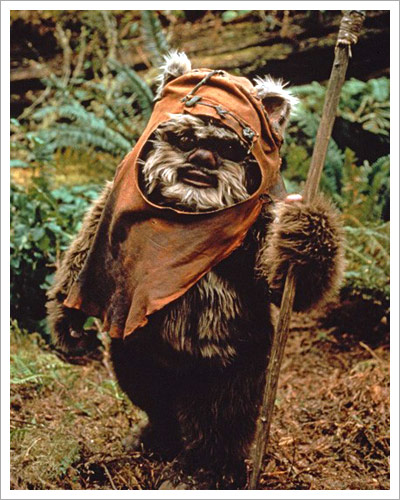
\includegraphics[scale=0.12]{ewok.jpg}}
    \column{0.2\textwidth}
      \uncover<3->{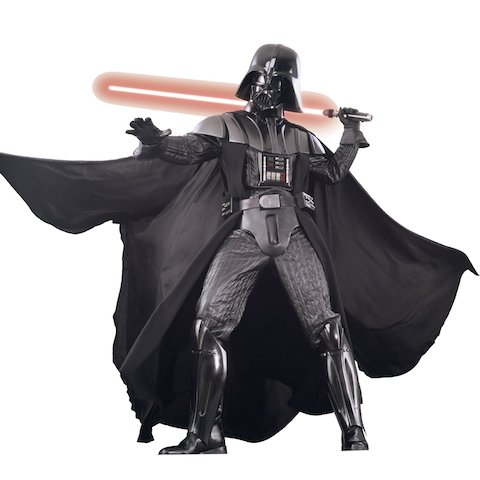
\includegraphics[scale=0.18]{vader.jpg}}

  \end{columns}
  
\end{frame}

\end{document}
